\begin{figure}
	% trim syntax order - {Left Bottom Right Top}
	{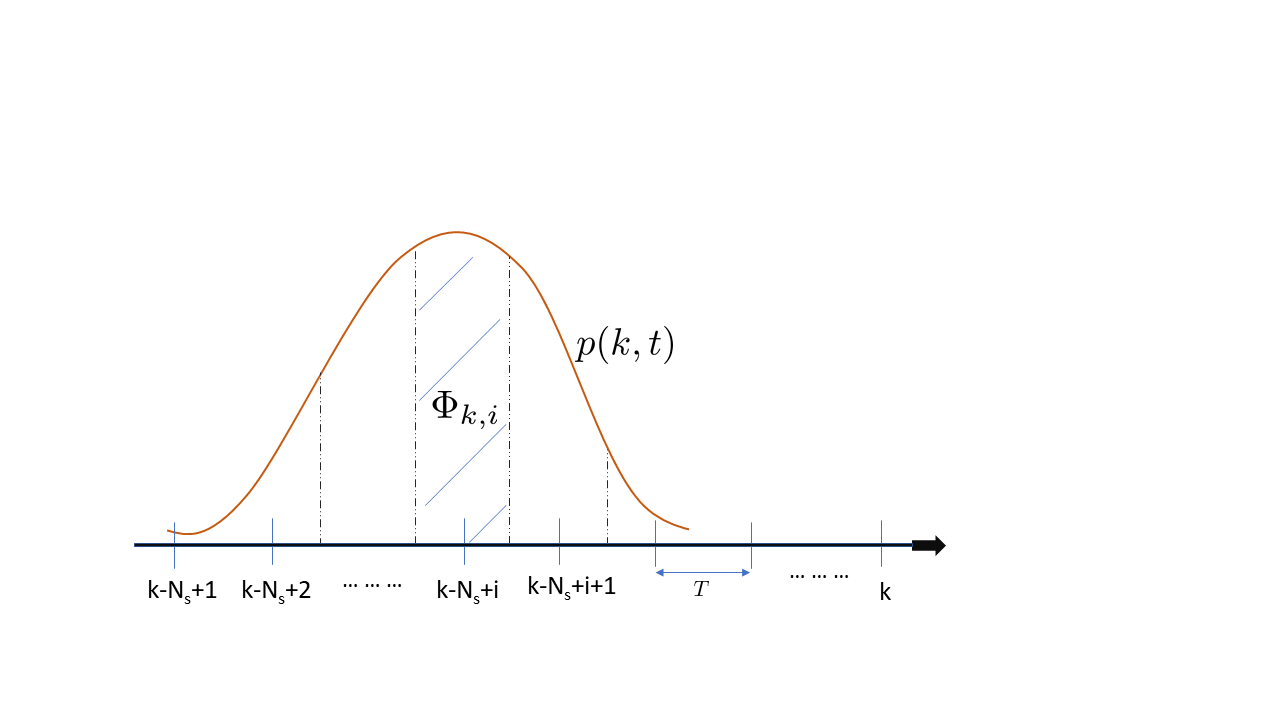
\includegraphics[trim={2.0cm 2.5cm 6.0cm 6.0cm},clip, width=\columnwidth]{./img/delay_uncertainty.png}}
	\caption{Uncertianty of delay}
	\label{fig:delay_uncertainty}
\end{figure}

This section will describe the state estimation approach for the linear system in eqns. (\ref{eqn:LinearStateProp}-\ref{eqn:LinearUndelayedMeasurement}), where the time-delayed measurements modeled in eqn. (\ref{eqn:LinearDelayedMeasurement}),  are corrupted by unknown bias $\Boldb_k$. 
For the derivation of the approach described in this section the reader is advised to refer to \red Section IV in \cite{choi2012state}.\black

\todo{AN: I commented out the text about augmenting the state-space model.  It should not be here as it is outside the scope of the section. Describe the augmented model in Section \ref{sect:applic}.}
%For the updated state vector, the linear time propagation model of eqn. (\ref{eqn:LinearStateProp}) can be rewritten as
%\begin{align}
%	\label{eqn:LinearStateProp4UpdatedState}
%	\Boldx_{k+1} &\doteq \BoldF \Boldx_k + \BoldGamma \Boldw_k,
%\end{align}
%the linear measurement models in eqns. (\ref{eqn:LinearDelayedMeasurement}) and (\ref{eqn:LinearUndelayedMeasurement}) can be rewritten as
%\begin{align}
%	\label{eqn:LinearDelayedMeasurement4UpdatedState}
%	\Boldz_k &\doteq \Big[ \BoldH_{k-N} \ \ \BoldI_{m_d} \Big] \Boldx_{k-N} +\Boldzeta_k \\
%	\label{eqn:LinearUndelayedMeasurement4UpdatedState}
%	\Boldy_k &\doteq \Big[ \BoldC_k \ \ \0_{m_u \times m_d} \Big] \Boldx_k + \Boldeta_k
%\end{align}

\blue\todo{AN: I revised the blue text. Please check. }
The probability density function (PDF) $p(t)$ of the delay is assumed to be a known and to  span over $\check{N}$ time steps.
An example pdf is shown in \red figure (\ref{fig:delay_uncertainty}). \blue 
Let $r(k,i)$ denote the event that measurement $\Boldz_k$ {\em corresponds} with $\Boldx_{k-\check{N}+i}$, $\forall i \in \{0, \dots, \check{N}\}$. 
The pdf $p(t)$ assigns a probability to each such correspondence of the delayed measurement $\Boldz_k$ with each of the time steps $j\in[k- \check{N},k]$.
The probability of correspondence $r(k,i)$ is computed as
\begin{align}
	\Phi_{k,i} &= Pr(r(k,i)) \\
	&= Pr(t_l \le t \le t_u) \\
	&= \int_{t_l}^{ t_u} p(t) dt,
\end{align}
where 
$t_l = {jT - \frac{T}{2}}$, 
$t_u = {j T + \frac{T}{2}}$, 
$j = k - \check{N} + i $,
$Pr(\cdot)$ denotes probability, and 
$p(\cdot)$ denotes the pdf of the time delay. 
When the PDF of the delay is specified, the maximum delay $\check{N}$ can be calculated using the cumulative distribution function (CDF) of the PDF. 
A value of $\check{N}$ should be chosen such that CDF of the time delay exceeds a given threshold. \black
In \cite{choi2012state}, Choi et. al. have shown that probability of the correspondence $r_i$ for the given measurement $\Boldz_k$ is\todo{AN: At this point, I can no longer revise. There is not enough detail for me to sort it out.}
\begin{align}
	P(r(k,i) | \Boldz_k ) = P(r(k,i)) = \Phi_{k,i}
\end{align}

Then, the optimal state estimator is
\begin{align}
	\hat{\Boldx}_k = \sum_{i=0}^{\check{N}} \Phi_{k,i} \hat{\Boldx}_{k,i},
\end{align}
where $\hat{\Boldx}_{k,i}$ is the estimation posterior computed the state estimate $\hat{\Boldx}_j^+$ computed in eqn. (\ref{eqn:posterior_state_estimate}), where $j = k - \check{N} + i$.

The optimal covariance matrix of the estimate is
\begin{align}
	\BoldP_k = \sum_{i = 0}^{\check{N}} \Phi_{k,i} [\BoldP_{k,i} + \hat{\Boldx}_k \hat{\Boldx}_k^\top] - \hat{\Boldx}_k \hat{\Boldx}_k^\top	
\end{align}
where $\BoldP_{k,i}$ is $a~posteriori$ state covariance matrix $P_j^+$ computed in eqn. (\ref{eqn:posterior_state_covar}),  where $j = k - \check{N} + i$. $\check{N}$



